\documentclass[12pt]{{memoir}}
\usepackage{graphicx}
\usepackage[overlay]{textpos}
\usepackage[hidelinks,pdfusetitle]{hyperref}
\usepackage{xfrac}
\usepackage[paperwidth=7.5in,paperheight=10.0in,top=.5in,bottom=.5in,left=.25in,right=.25in]{geometry}

\newcommand\Hline{%
\hline\raisebox{0pt}[1.125em]{}}


\interfootnotelinepenalty=10000
\begin{document}
\title{Retro 6k Emulator User's Guide}
\author{Maggie\,David P.\,K. Haynes}
\pagestyle{empty}
\begin{center}
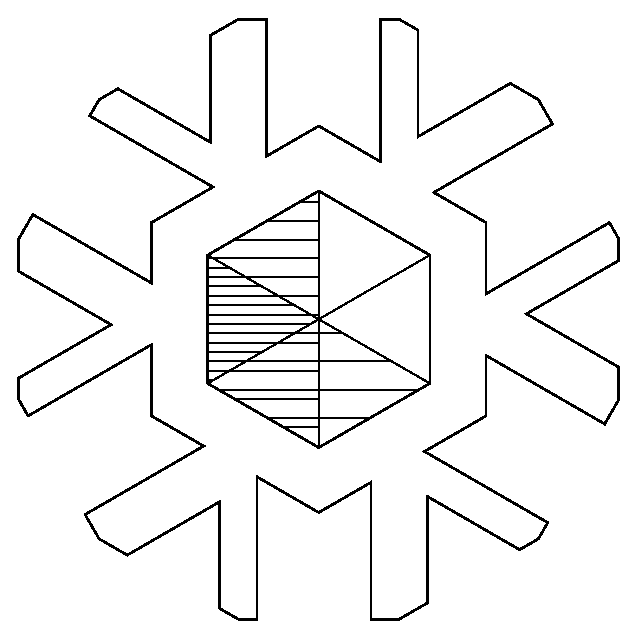
\includegraphics{../common-src/logolineart}

\vspace{\stretch{.25}}
{\sffamily\bfseries\Huge{}Retro 6k\\Fantasy Computer\\Entertainment System

\vspace{\stretch{1}}
Emulator User's Guide\par}
\vspace*{\stretch{1}}
{\sffamily\bfseries\large\theauthor\par}
\end{center}
\vspace*{\stretch{3}}
\cleartoverso
\vspace*{\stretch{2}}
\begin{center}
\noindent{}Here's where I\\
write a personal note...\par
\end{center}

\vspace*{\stretch{3}}
\cleartorecto
\tableofcontents*
\clearpage
\pagestyle{headings}

\vspace*{3in}
\section*{Conventions Used In This Document}

Nothing established yet.

\chapter{Configuration}

\section{Configuration File}
\label{sec:configfile}

\subsection{Location}
\label{ss:configloc}

In Windows, the first place the Retro 6k emulator looks for configuration data is the Windows Registry, where the format of the configuration data is a little different than in a file on disk. On Unix/Linux systems, the emulator first looks for a file at \texttt{/etc/.retro6k-config}. If not found, the emulator will next look for a file called \texttt{.retro6k-config} in the current user's home directory. Failing that, the emulator will finally look for a file called \texttt{.retro6k-config} in the same directory as the emulator's own executable file. However, if the emulator is launched with a command line option specifying where to look for configuration data, the emulator will look there and only there.

\subsection{Format (on disk)}

The configuration file on disk is divided into sections. Each section begins with a line consisting of the name of the section in square brackets, like this: \texttt{[foo]}. Within each section, each line declares a key/value pair. The first \texttt{=} on a line is interpreted as a separator; everything to the left is the key, while everything to the right is the value. Any line that begins with a \texttt{\#} is interpreted as a comment and disregarded.

\subsection{Format (in Windows Registry)}

Formatting of configuration data in the Windows Registry remains to be determined.

\subsection{\texttt{[paths]} section}

Four keys are recognized in the \texttt{[paths]} section: \texttt{cart}, \texttt{rom}, \texttt{save}, and \texttt{screencap}. Each line adds the given value as a filesystem path to the list of preset paths to use to load or save files of the category given as the key. Multiple paths can be declared for each category, simply by writing multiple lines that start with the same category key. At the beginning of any path value, the character \texttt{\#} will expand to the location of the emulator's executable file, and the character \texttt{\raisebox{-.25em}{\textasciitilde}} will expand to the user's home directory. The first entry in each path list is the one used by default when a file open or save dialog is activated. Note that paths given on the command line take precedence over paths read from the configuration file.

\subsection{\texttt{[screen]} section}

\begin{center}\begin{tabular}{>{\ttfamily}lll}
\textrm{Key} & Value & Description \\
\Hline
aspectratio & \texttt{classic} & Aspect ratio is reported to software as 4:3.\\
& \texttt{free} & Aspect ratio is determined automatically.\\
& \texttt{wide} & Aspect ratio is reported to software as 16:9.\\
pixheight & \texttt{auto} & The height of the emulated display is chosen to fit the screen.\\
& \textit{number} & Each emulated pixel is displayed \textit{number} screen pixels tall.\\
pixwidth & \texttt{auto} & The width of the emulated display is chosen to fit the screen.\\
& \textit{number} & Each emulated pixel is displayed \textit{number} screen pixels wide.\\
& & If one or both of \texttt{pixheight}, \texttt{pixwidth} are \texttt{auto}, and \\
& & \texttt{aspectratio} is set to \texttt{classic} or \texttt{wide}, then the display \\
& & aspect ratio is constrained accordingly.
\end{tabular}\end{center}

\section{Command Line Arguments}

The name of the Retro 6k emulator executable file may differ from system to system. Currently, on Windows it's \texttt{retro6k.exe} while on Unix/Linux systems it's simply \texttt{r6k}. A cartridge file name may be specified before, amidst, or after other options, and the emulator will load that cartridge on startup rather than prompting the user to select a cartridge. A cartidge instance (save) file name may be specified after a cartridge file name, with or without options in the interim, and the emulator will load that cartridge instance after loading the cartridge, rather than prompting the user to select an instance. Multiple short options (switches) may be combined after a single hyphen, but only the last of them can have a parameter specified after it.

\begin{center}
Syntax: (\texttt{retro6k}\textbar\texttt{r6k}) [\textit{options}] [\textit{cartridge} [\textit{options}] [\textit{instance}]] [\textit{options}]

\vspace{1em plus 1em minus 1em}

\begin{tabular}{>{\ttfamily}l>{\ttfamily}ll}
\textrm{Switch} & \textrm{Option} & Description \\
\Hline
-p \textrm{\textit{dir}} & --cartpath \textrm{\textit{dir}} & Specifies a path in which cartridges may be found. Only one \\
& & path may be specified. Use multiple \texttt{--cartpath} options to \\
& & specify multiple paths. \\
-c \textrm{\textit{file}} & --configfile \textrm{\textit{file}} & Specifies location of config file to use. Overrides built-in \\
& & config file search paths as described in section \ref{sec:configfile} on page \pageref{ss:configloc}. \\
-r \textrm{\textit{dir}} & --rompath \textrm{\textit{dir}} & Specifies a path in which system ROM images may be found. \\
& & Only one path may be specified. Use multiple \texttt{--rompath} \\
& & options to specify multiple paths. \\
-s \textrm{\textit{dir}} & --savepath \textrm{\textit{dir}} & Specifies a path in which cartridge instance (save) files may \\
& & be found and/or saved. Only one path may be specified. Use \\
& & multiple \texttt{--savepath} options to specify multiple paths. \\
& --screencappath \textrm{\textit{dir}} & Specifies a path in which screen captures should be saved.\\
\end{tabular}
\end{center}

\chapter{Startup}

When the Retro 6k emulator starts, the first thing it does is ask which cartridge to ``insert''. If you press \textsf{Esc}, the cartridge selection closes and the system boots without a cartridge inserted. If you do select a cartridge, the emulator may then ask you to choose which ``instance'' or ``save'' of the selected cartridge to load; the physical equivalent is which of multiple copies of a cartridge are inserted into the machine. This will only happen if the selected cartridge is designed to store data persistently. The process is described in greater detail in chapter \ref{ch:cartridges} on page \pageref{ch:cartridges}. Following the selection of a cartridge and possibly an instance file, the system boots with the selected cartridge inserted.

\chapter{Menu}

[TODO]

\chapter{Cartridges and Saves}
\label{ch:cartridges}

[TODO]

\cleartoverso
\pagestyle{empty}
\vspace*{\stretch{1}}

\noindent\thetitle\hfill\textcopyright2019--20 \theauthor

\end{document}
